\section{Control}
\label{sec:control}


\subsection{Overview of Control Strategy}
\label{sec:overview}

In this work, I rely on \emph{optimal control} formulation to design an efficient locomotion controller. The resulting motion is optimal w.r.t. the desired criteria, which can be expressed as an objective function and constraint(s). A high level specification (such as minimizing energy, tracking a desired foot trajectory, tracking a desired torso angle) can be translated quite easily to the objective function. 

However, there are several challenges in implementing the optimal controller to this problem. Firstly, most optimal control strategy in robotics is time-based. That is, the time horizon has to be specified (e.g. 1 second), and solving the optimal control problem will give us a specific control and state trajectory for this time horizon that minimizes the objective function while satisfying the constraints. Some variants are time independent, e.g. when the time horizon is infinite, but it is not suitable for this locomotion problem (where the desired behavior highly depends on time and event, and not stationary). Since the impact timing is difficult to predict precisely (especially given some disturbance), a purely time-based controller is difficult to be used here. Secondly, the dynamics model of our locomotion is discontinuous due to the impact map. This is a big problem for optimal control, as most methods would require the gradient of the dynamics function. 

To overcome these issues, I propose to use the following approach. First, the optimal control is solved for only one step until impact, so that the discontinous event at the impact is not considered. Considering that the locomotion is a periodical motion, designing an optimal trajectory for one step should be sufficient, provided that the state after the impact returns to the initial state. 
Secondly, we need a controller that is not purely time based or feed forward only. One option is to use a feedback controller (e.g. PD) to track the desired optimal trajectory. However, there is a specific optimal control formulation that provides this automatically, i.e. Iterative Linear Quadratic Regulator (ILQR)~\cite{Tassa2012}. Solving ILQR gives us both the optimal trajectories and the optimal feedback controller (note that 'optimal' here refers to local optimum, not the global one). 
Finally, to choose the optimum parameters for the optimal control, we again rely on an optimization solver (fmin) to ensure that the controller is stable.

\subsection{Iterative Linear Quadratic Regulator (ILQR)}
\label{sec:ilqr}

A general discrete Optimal Control Problem consists of a cost function
\begin{equation}
C(\bm{x}, \bm{u}) = \sum_{t=0}^{T-1} c_t(\bm{x}_t, \bm{u}_t) + c_T(\bm{x}_T, \bm{u}_T),
\label{eq:general_cost}
\end{equation}
subject to the dynamics
\begin{equation}
\bm{x}_{t+1} = \bm{f}(\bm{x}_t, \bm{u}_t).
\label{eq:general_dynamics}
\end{equation}
$(\bm{x}, \bm{u})$ are the state and control trajectories for the time horizon $T$. $\bm{x}_t$, the state at time $t$, consists of the joint angles and velocities, i.e. $\bm{x}_t = [\bm{q}_t, \dot{\bm{q}_t}]$.  ILQR solves this optimal control problem by iteratively formulating a sub problem as a Linear Quadratic Problem (LQR) problem and solve it to obtain a better solution at each iteration.

Let us consider the current guess $(\bm{x}^k, \bm{u}^k)$, where $k$ is the iteration index. Given the general cost function in \eqref{eq:general_cost}, we approximate it as a quadratic function around $(\bm{x}^k, \bm{u}^k)$,
\begin{multline} 
\hfill
\centering
c_t(\delta\bm{x}_t, \delta\bm{u}_t) = \frac{1}{2} 
\begin{bmatrix}
\delta \bm{x}_t \\ \delta \bm{u}_t 
\end{bmatrix}
^\trsp
\begin{bmatrix}
\bm{c}_{\bm{xx},t} & \bm{0} \\ \bm{0} & \bm{c}_{\bm{uu},t}
\end{bmatrix}
\begin{bmatrix}
\delta \bm{x}_t \\ \delta \bm{u}_t 
\end{bmatrix}
 + 
\begin{bmatrix}
\bm{c}_{\bm{x},t} &  \bm{c}_{\bm{u},t}
\end{bmatrix}
\begin{bmatrix}
\delta \bm{x}_t \\ \delta \bm{u}_t 
\end{bmatrix},
\label{eq:quadratized_cost}
\end{multline}
where $\bm{c}_{\bm{x},t}, \bm{c}_{\bm{u},t}, \bm{c}_{\bm{xx},t},$ and $\bm{c}_{\bm{uu},t}$ are the cost function's first and second order derivatives with respect to $\bm{x}$ and $\bm{u}$. Similarly, we can approximate the dynamics in \eqref{eq:general_dynamics} using the linear approximation
\begin{equation}
\delta \bm{x}_t = \bm{A}_t \delta \bm{x}_t + \bm{B}_t \delta \bm{u}_t,
\label{eq:linearized_dynamics}
\end{equation}
where $\bm{A}_t$ and $\bm{B}_t$ are the derivatives of the dynamics $\bm{f}(\bm{x}_t, \bm{u}_t)$ with respect to $\bm{x}_t$ and $\bm{u}_t$, respectively. The derivatives are evaluated at the current guess $(\bm{x}^k, \bm{u}^k)$. With this, we have quadratic costs and linear dynamics as functions of $\delta\bm{x}$ and $\delta\bm{u}$. This is therefore a time-varying LQR problem, of which the variables of interest are $\delta\bm{x}$ and $\delta\bm{u}$, and the solution can be computed analytically. 

By the end of ILQR iteration, we will have a locally optimal solution as state and control trajectories $(\bm{x}^*, \bm{u}^*)$, as well as the time-varying optimal feedback term $\bm{K}_t$. To use this feedback term, at online execution we compute the control command by 
\begin{equation}
\bm{u}_t = \bm{u}_t^* + \bm{K}_t (\bm{x}_t - \bm{x}_t^*).
\end{equation}
This optimal feedback term serves as a locally optimal PD controler to track the optimal trajectories $(\bm{x}^*, \bm{u}^*)$. 

More details about ILQR can be found in ~\cite{Tassa2012}. 

\subsection{ILQR formulation for the locomotion}
For the locomotion problem, we consider the initial state $\bm{x}_0$ to be the state right after an impact, and the end state $\bm{x}_T$ to be at the next predicted impact. It turns out that formulating the objective function for this problem is quite complicated, especially due to the fact that the impact is detected based on event, and cannot be predicted too precisely by the timing. I previously try using an objective function to only reach the desired end state $\bm{x}_T$, but this often results in failure because the swing foot touches the ground before reaching $\bm{x}_T$. In this event based detection, the swing foot trajectory is very important. Another variable that is also important is the torso angle ($\bm{q}_3$). This needs to be regulated carefully, otherwise the motion is often unstable. 

After a lot of trials, the objective function that is found to be working is to track a desired foot swing trajectory, while keeping the torso angle to be around a desired angle. The running cost, i.e. the cost for $t = [0, T-1] $ is set to be
\begin{equation}
c(\bm{x}_t, \bm{u}_t) = (\bm{r}_{swf, t} - \bm{r}_{swf, t}^*)^\trsp \bm{W} (\bm{r}_{swf,t} - \bm{r}_{swf, t}^*) + \lambda (q_{3,t} - \alpha)^2 +  \bm{u_t}^T \bm{R} \bm{u}_t,
\end{equation}
while the terminal cost at $t = T$ is set to be 
\begin{equation}
c(\bm{x}_T, \bm{u}_T) = (\bm{r}_{swf, T} - \bm{r}_{swf, T}^*)^\trsp \bm{W}_T (\bm{r}_{swf, T} - \bm{r}_{swf, T}^*) + \lambda (q_{3,T} - \alpha)^2.
\end{equation}

The constraint on the control input is a box constraint, 
\begin{equation}
-30 \leq \bm{u}_i \leq 30 \quad \text{for} \quad  i = 1, 2 . 
\end{equation}

For time $t < T$, we only care about its vertical coordinate $z_{swf}$, to make sure that it does not touch the ground before time $T$. I use a simple linear interpolation between the initial height $z_{swf,0}$ and final height $z_{swf,T}$. At time $t=T$, we want the swing foot to reach a specific foot location, so both the horizontal and vertical coordinates are important. The horizontal coordinate corresponds to the desired step length, while the vertical coordinate corresponds to the ground (in this case, around ~$-0.01$). The weight parameters are
\begin{equation}
\bm{W}_t = \begin{bmatrix}
0 & 0 \\ 0 & 10^4  
\end{bmatrix}, 
\bm{W}_T = \begin{bmatrix}
10^4 & 0 \\ 0 & 10^5  
\end{bmatrix}, 
\bm{R} = \begin{bmatrix}
10^{-2} & 0 \\ 0 & 10^{-2}  
\end{bmatrix}, 
\lambda = 100.
\end{equation}   

To solve this constrained ILQR problem, I use the open source solver Crocoddyl~\cite{Mastalli}. It uses the box-FDDP algorithm~\cite{mastalli2020direct} that accepts infeasible initial guess $(\bm{x}^0, \bm{u}^0)$. \emph{Infeasible} here means that $(\bm{x}^0, \bm{u}^0)$ may not be dynamically consistent. Allowing this infeasibility makes the initialisation easy. 

\subsection{Optimization Strategy}
\label{sec:opt_strat}

To use the optimal control formulation, we have to choose the following parameters $\bm{\Phi}$:
\begin{itemize}
\item The initial state $(\bm{q}_0, \dot{\bm{q}_0})$
\item The desired torso angle $\alpha$
\item The desired goal position for the swing foot $x_{swf,T}^*$
\end{itemize}

In addition, we also have to specify the time horizon $T$. Although optimal control formulation is powerful, finding the optimal parameters for a desired objective of this particular locomotion problem turns out to be challenging. Instead of starting from random initial guess, I rely on the standard controller discussed in Section~\ref{sec:control_opt}. For a given desired criteria (e.g. a desired speed, step length etc.), first I optimize this standard controller to achieve the criteria, and observe the corresponding parameters $\bm{\Phi}$ as well as the time interval $T$. Using this with the ILQR often results in failure, i.e. unstable controller, as the ILQR is still time based and depend a lot on the impact event. So we need to further optimize $\bm{\Phi}$ to obtain a good controller.

To make the optimization tractable, I do it step by step. First, I optimize for only one foot step. Since a stable controller will have a stable limit cycle, the next state after the impact should be very close to the initial state. So I design the objective function for the optimization to be 
\begin{equation}
f(\bm{\Phi}) = ||\bm{x}_0 - \bm{x}_T^+ ||_2,
\end{equation}
where $\bm{x}_0$ is the initial state, and $\bm{x}_T^+$ is the final state after the impact (i.e. the initial state for the next foot step). By ensuring that $\bm{x}_0$ is as close as possible to $\bm{x}_T^+$, we can have a stable limit cycle. 

In practice, optimizing for only one foot step sometimes makes a stable controller for only a few foot steps, as the error diverges. When this happens, the optimization is run again, but this time with a longer foot steps, and initialized using the previously obtained parameters. Doing this iteratively often results in a controller that is stable for a large number of foot steps, even to infinity. 

\subsection{Results and Discussion}
\label{sec:results}

Table~\ref{tab:ilqr_result} shows the parameters for the ILQR controller for various criteria. The parameters for the extreme value of one criteria turns out to yield another extreme value of another criteria, hence the same parameters $\bm{\Phi}$. For example, the controller for maximum velocity here also yield the largest step length in our experiment. 

Here we note that the step length predicted by the ILQR controller may not correspond to that happen during the simulation, due to the feet touching the ground before that. This is the case for the minimum step length (0.117 m). The desired step length input to the controller is 0.25, but the interaction between the controller and the actual system results in a different motion, which looks quite interesting (it can be seen in the supplementary video). Fig.~\ref{fig:ilqr_plot} shows the plots of various variables of interest for the controller with velocity = 0.877 m/s. 

\subsubsection{Internal and External Perturbation}
I do not have time to run the optimization for handling the perturbation, so I just try the controller with the parameters that I find most stable qualitatively. While playing with the optimization, I often observe that the motion is quite stable when the velocity is around ~0.8m/s, so I optimize the ILQR controller around this speed. I obtain the parameters as $\bm{q}_0 = (-0.275,  0.319,  0.192),\dot{\bm{q}_0} = (0.774, -0.874,  4.05), \alpha = 0.189, \text{step length} = 0.302, T = 0.382$.

With these parameters, the maximum internal perturbation is $\sigma_q = [0.1, 0.15, 0.1 ], \sigma_{qd} = [3, 2, 1.2]$", where $\sigma_q$ and $\sigma{qd}$ are the noise standard deviation for the joint angles and velocities, respectively. Note that the controller is more sensitive towards the error in the joint angle estimation as compared to the velocity. The noises are also limited at $\pm 3\sigma$. The allowable external perturbation, in the form of horizontal force at the hip, is $F = [-51, 18] N$. 

We note here that ILQR controller is not particularly robust towards large perturbation. The feedback gain $\bm{K}_t$ is only optimal and valid near the optimal trajectory $(\bm{x}^*, \bm{u}^*)$. To perform more stably, one possible idea is to track the optimal trajectory using another controller, e.g. PD controller, or Quadratic Programming (QP) controller as in~\cite{park2017high}. I have tried implementing this, but I did not have time to find the good parameters for the QP. 

Another possible approach is to recompute the ILQR at each iteration in Model Predictive Control (MPC) fashion. This will give good result and possibly the most stable. However, this requires a lot of computational time, and I cannot make the computation time below 1ms as would be required here. In our implementation, the ILQR requires ~100ms for 1 iteration. A hierarchical controller may be an option, i.e. when the MPC is computed at slower frequency (e.g. 100 Hz). 


\renewcommand{\arraystretch}{1.}
\begin{table}[h!]
	\centering    
      \caption{Parameters for ILQR controller}
      \label{tab:ilqr_result}
		
	\begin{tabular}{l l | c  c  c c c}
		\toprule
\bf{Criteria} & \bf{Value} & $\bm{q}_0$ & $\dot{\bm{q}_0}$ & $\alpha$ &  \bf{Step} & $T$\\
\bf{Vel} & 0.31 & (-0.17,  0.27,  0.05) & (  1.8 ,  0.99,  0.02) &   0.05 & 0.25 & 0.268 \\
\bf{Vel} & 0.877 &( -0.34,  0.39,  0.35) & (  0.78, -1.45,  5.44) &   0.34&       0.36 & 0.421\\
\bf{Freq} & 2.2 & (-0.34,  0.39,  0.35) & ( 0.79, -1.45,  5.44) &   0.34&0.36 &0.421  \\
\bf{Freq} & 3.65 & (-0.17 ,  0.27 ,  0.05) & (  1.84,  0.99,  0.02) &   0.05 &        0.25 &0.268 \\
\bf{Step} & 0.117 &(-0.17,  0.27,  0.05) & (  1.84 ,  0.99,  0.02) &  0.05& 0.25& 0.268\\
\bf{Step} & 0.372 &(-0.34,  0.39,  0.35) & (  0.79, -1.45,  5.44) &   0.34& 0.36& 0.421 
	\end{tabular}
\end{table}




\begin{figure}
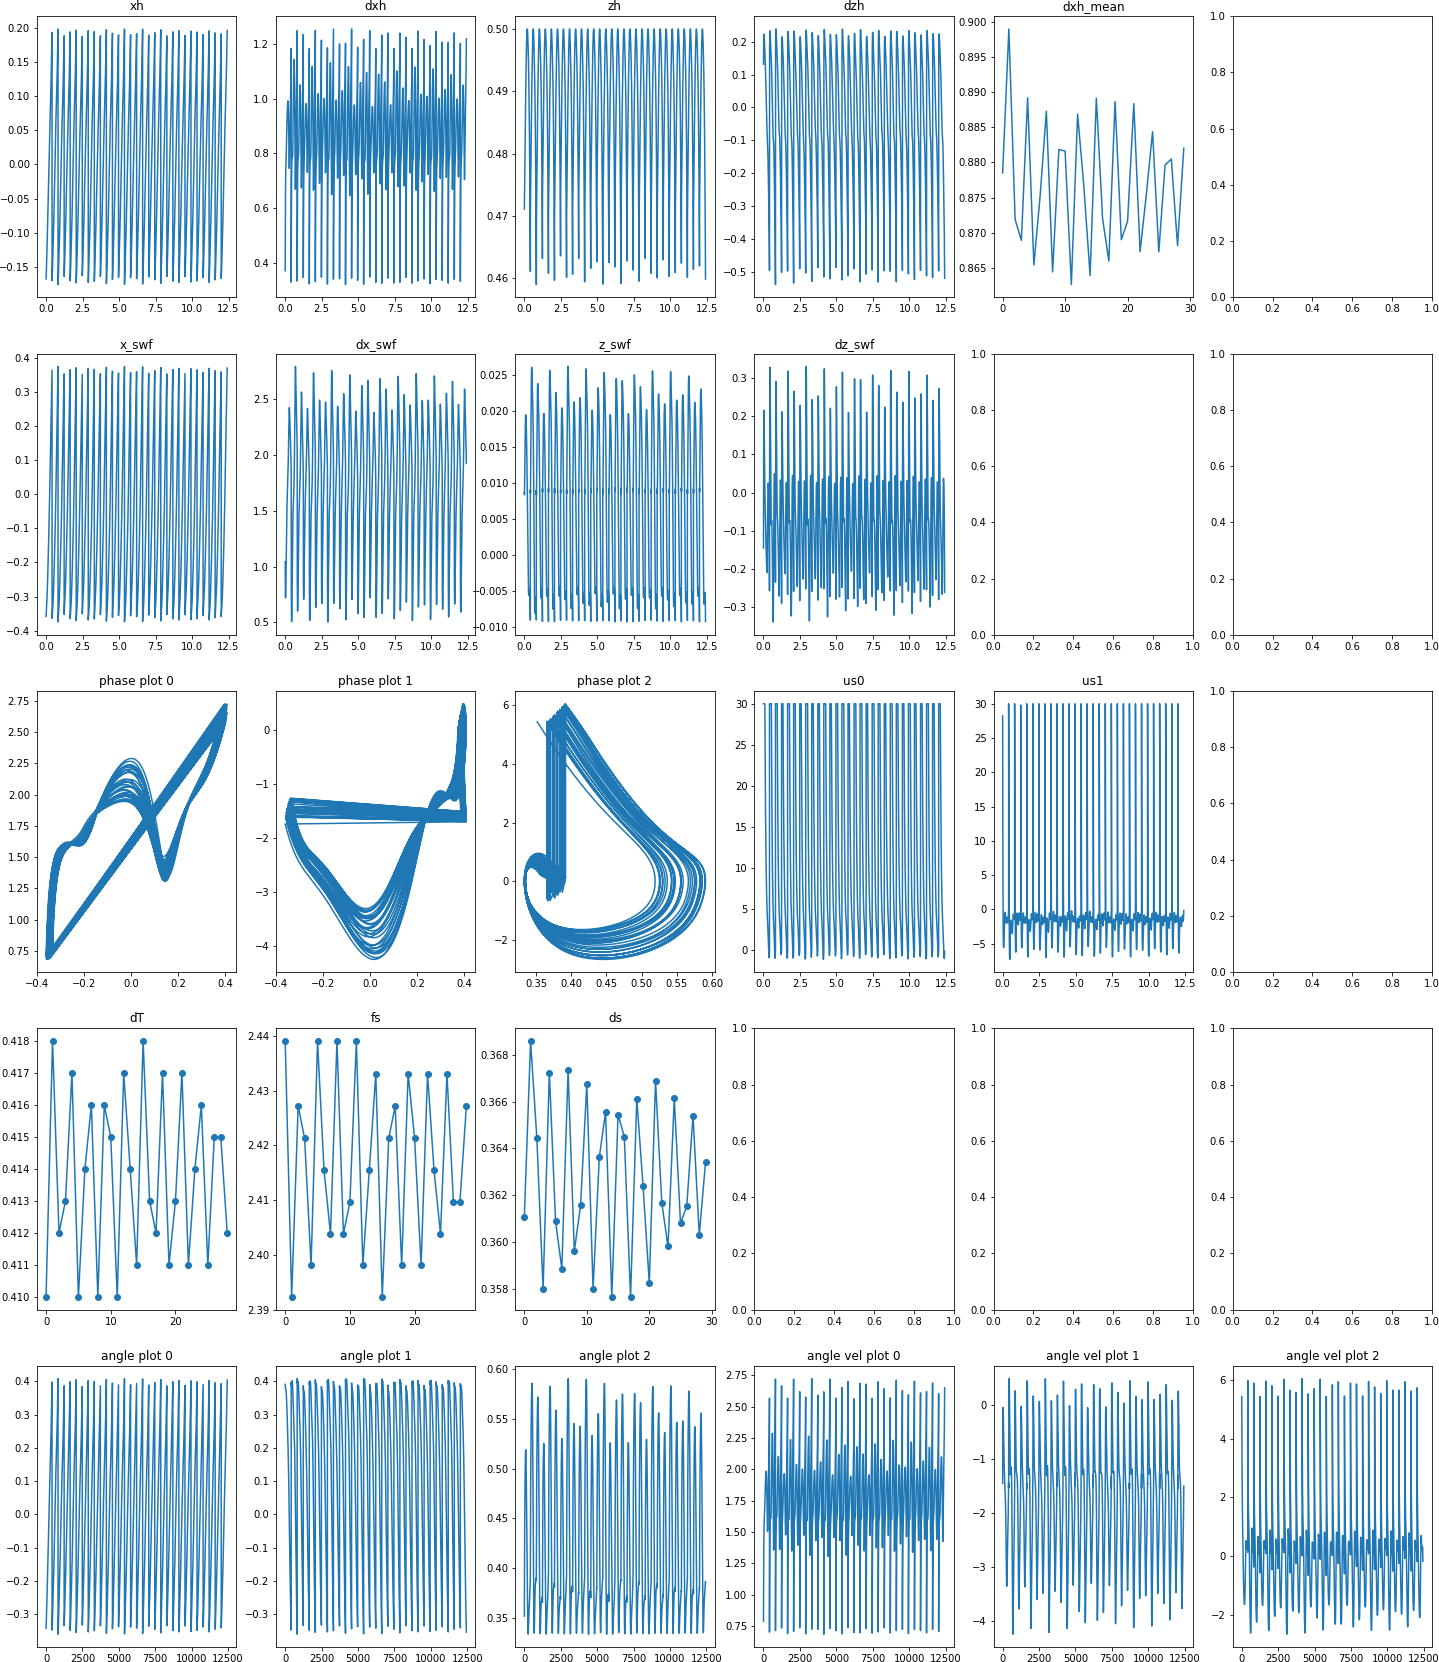
\includegraphics[width=0.99\columnwidth]{example_v09_prev}
\caption{Various plots for the ILQR controller simulation with velocity = 0.877}
\label{fig:ilqr_plot}
\end{figure}

